%!TEX root = main.tex
\section{Neutron Attenuation In Water} % (fold)
\label{sec:neutron_attenuation_in_water}

\subsection{Boron Tri-Flouride Detector} % (fold)
\label{ssub:boron_tri_flouride_detector}
The BF$_3$ detector is a proportional counter. It contains boron trifluoride gas at 0.5 to 1 atmospheres which acts as both a target for slow neutron conversion into secondary particles, as well as a proportional gas. A large potential difference is applied across the gas. The cathode which is held at ground is the outer tube of the detector and is generally made from aluminium since this has a low neutron absorption cross section so should not influence any readings made by the detector. The anode, at high voltage, is a single wire that passes through the centre of the detector, see figure~\ref{fig:bf3detector}. When a neutron is incident in the reactor, one of the reaction below takes place\cite{krane}.
\begin{align}
	\cf{^{10}_{5}B} + \cf{^{1}_{0}n} &\rightarrow \cf{^{7}_{3}Li} + \cf{^{4}_{2}\alpha} \label{eq:bf31}\\
	\cf{^{10}_{5}B} + \cf{^{1}_{0}n} &\rightarrow \cf{^{7}_{3}Li^*} + \cf{^{4}_{2}\alpha} \label{eq:bf32}
\end{align} 

The products of these two equations differ only by the energy of the lithium which, in some cases, is left in an excited metastable state with a slightly different energy. The relative probabilities of each reaction is 96\% for equation~\ref{eq:bf31} and 4\% for equation~\ref{eq:bf32}\cite{baratta}. The resulting ions that are created are attracted to the poles of the detector and so provide a voltage through it. This provides a signal which is sent to the processing computer. It should be noted that this detector cannot give any information of the energy of the neutron since the formation of the ions is independent of energy over a certain level. Instead, this detector is used simply as a counter to obtain a value for the number of neutrons hitting it in a specified time period. 
\begin{figure}[ht]
	\centering
	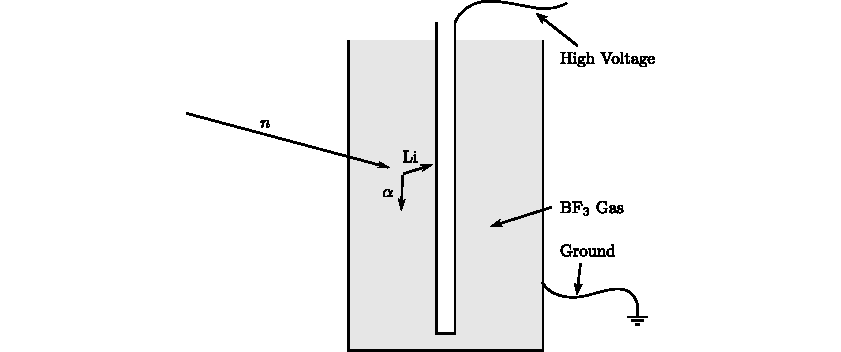
\includegraphics[width=0.9\textwidth]{BF3detector.pdf}
	\caption{The $\text{BF}_4$ detector uses a high charge to create a flow of ions to measure the incoming neutron. It cannot measure the energy, but simply gives a count for the number of neutrons incident in the detector. The anode and cathode create a large electric field inside the detector that creates the flow of charge used to count the incoming particles.\label{fig:bf3detector}}
\end{figure}

When the reaction happens, the products, $\cf{^{7}_{3}Li}$ and $\cf{^4_2\alpha}$, are ejected through the BF$_3$ gas at a high velocity and can go on to cause further reactions in the gas as these ions deposit their kinetic energy. The electric field close to the wire increases quickly ($E\propto\frac{1}{r^2}$) and so a Townsend avalanche forms near to the wire when a reaction occurs. This involves the electrons being accelerated greatly by the electric field which causes the gas to conduct through the avalanche. The avalanche terminates when all of the free electrons reach the anode. These electrons produce the signal which is measured by the computer and used for analysis. Despite the several steps involved, if the detector is well designed, the number of electrons that is measured can be ensured to be proportional to the incident energy of the particles\cite{krane}.

\subsubsection{Wall Effect} % (fold)
\label{ssub:wall_effect}

The BF$_3$ detector shall be used for several purposes later, so it is worth discussing some of the features of the data that is produced by this detector. Figure~\ref{fig:walleffect2} shows a typical spectrum from the BF$_3$ detector. This shows a main peak, a smaller, higher energy secondary peak and an example of the wall effect.

When a neutron is incident with one of the atoms in the gas in the reactor, one of the reactions equation~\ref{eq:bf31} or~\ref{eq:bf32} takes place. If the reactor was extremely large compared to the travel distance of the Li and $\alpha$ products, then a single peak from each of the reactions would be observed, along with some amount of background noise, giving a spectrum similar to the top graph in figure~\ref{fig:walleffect2}. The two peaks are from the reaction producing a ground state lithium atom or an excited lithium atom respectively. 
\begin{figure}[ht]
  \centering
  \begin{overpic}[width=0.8\columnwidth]{walleffect2.pdf}
    \put(57,48){2.31}
    \put(68,48){2.79}
    \put(25,25){Wall effect}
    \put(25,22){continuum}
    \put(30,20){\vector(0,-4){11}}
    \put(30,20){\vector(3,-2){12}}
    \put(65,40){$\text{Li}^* + \alpha$}
    \put(73,8){$\text{Li} + \alpha$}
    \put(46,12){$\alpha$}
    \put(32,9){Li}
  \end{overpic}
  \caption{An exemplar spectrum from the BF$_3$ detector showing the two peaks from each of the two reaction products, and the wall effect when one of the products from equation~\ref{eq:bf31} escapes the detector.\label{fig:walleffect2}}
\end{figure}

The two steps in the count number at lower channel numbers is known as the wall effect. These are due to the detector being finite, or small compared to the travel distance of the reaction products, and so there is a chance that one of the products from the reaction escapes from the detector. Due to the relative masses of the particles created, $\alpha$ and Li, the $\alpha$ particle takes most of the energy from the original neutron and so when it is lost from the detector, the recoded energy is lower\cite{krane}.

Other features of the spectrum are the abrupt cut-off at the low channel numbers. This is to reduce the background counts that are present in this region from obscuring the rest of the data. 
% subsubsection wall_effect (end)

\subsection{Using Water as a Neutron Moderator} % (fold)
\label{sub:using_water_as_a_neutron_moderator}
The typical neutrons that are created by the BeAm source have energies of several MeV. Since the energy and the temperature are related by the equation
\begin{align}
  E = \frac{1}{2}mv^2 &= \frac{3}{2}kT
\end{align}
This means that the neutrons have a temperature in the order of tens of millions of degrees kelvin. In any application where neutrons are a by-product, or not used directly, these speed can be dangerous to anything around the source. To alleviate this safety issue, a moderator is used, placed 360 degrees around the source to reduce the energy of the neutrons to a level that is safe to be near. Moderation is the action of reducing the kinetic energy of a neutron or other particle through collisions with other particles. 
% subsection using_water_as_a_neutron_moderator (end)

\subsubsection{Boron Triflouride Detector Set-up} % (fold)
\label{ssub:boron_triflouride_detector_set_up}
Since it is only a proportional counter, and so gives no information for the energy of the observed particles, there is no calibration to be done with the BF$_3$ detector. However, there is a certain degree of adjustment that can, and should, be made to the settings of the detector before proceeding with the data acquisition. The detector requires a high voltage of between 1.4 to 2.6\,keV. This is the safe working range, but inside these limits, the voltage that gives the clearest results can be chosen. Figure~\ref{fig:bf3voltages} shows several graphs from the BF$_3$ detector using different voltages to ascertain which would be the most appropriate voltage to use.
\begin{figure}[ht]
  \centering
  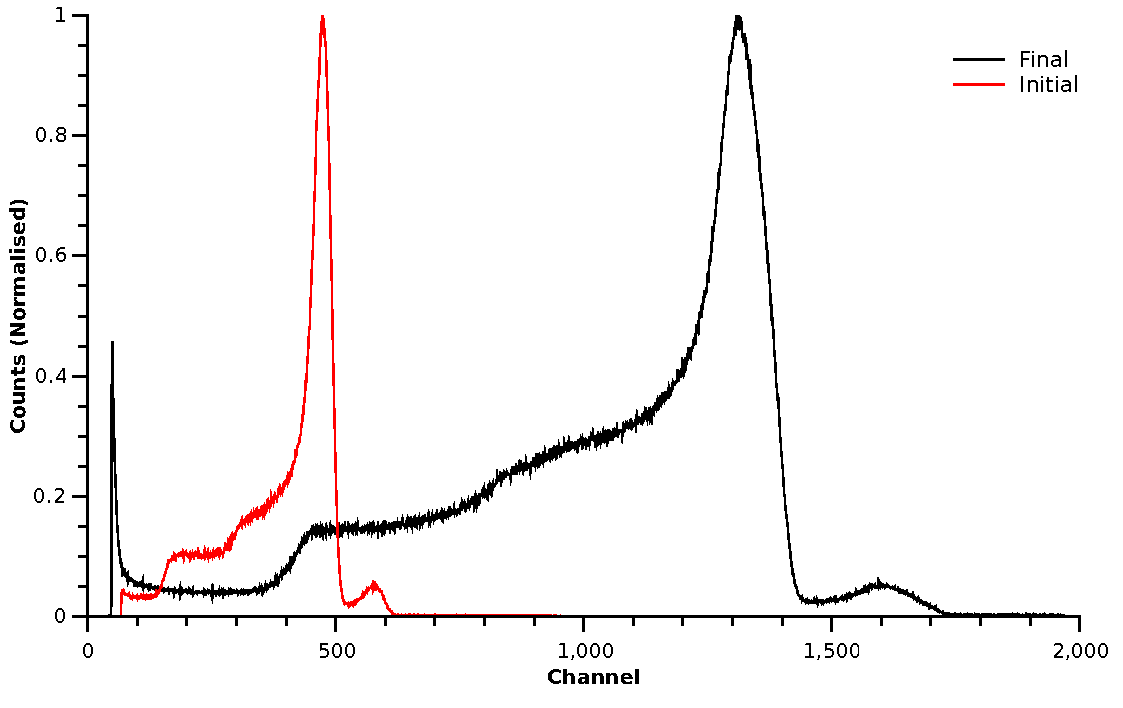
\includegraphics[width=0.6\textwidth]{BF3_calib_voltage.pdf}
  \caption{The effect of adjusting the supplied voltage correctly. The initial readings, using the lower bound of the allowed voltage range does not make full use of the channel range and so any readings will be subject to higher errors. The final voltage level that was used takes full advantage of the channel width of the detector. \label{fig:bf3voltages}}
\end{figure}
% subsubsection boron_triflouride_detector_set_up (end)

% subsubsection boron_tri_flouride_detector (end)
\subsection{Neutron Attenuation} % (fold)
\label{sub:neutron_attenuation}In order to examine the attenuation effects of water to neutrons from the beryllium-americium source, the spectrum of neutrons will be measured with the BF$_3$ detector at a range of distances from the source, moving radially outward through the water. The readings shall be taken for precisely the same length of time using the built in timing function of the software used to record the readings. The count value from the data will be taken from the centre of the lower wall upwards, since everything below this point must be background radiation.

An estimate for the background radiation involved in the main section of the readings can also be made. By looking at the spectrum recorded from the detector, it can be seen that the background level just prior to the first wall, and so before any useful information from either reaction, and just after the second peak, can be joined by a straight line, representing a linear falloff of background across the channels. This is shown in figure~\ref{fig:bf3errorest}. The count number represented by this triangle can be measured, and subtracted from the total count, which shall also be taken inside these limits. This should provide a reduced count number that has removed a significant proportion of the background that would have affected the result.
\begin{figure}[ht]
  \centering
  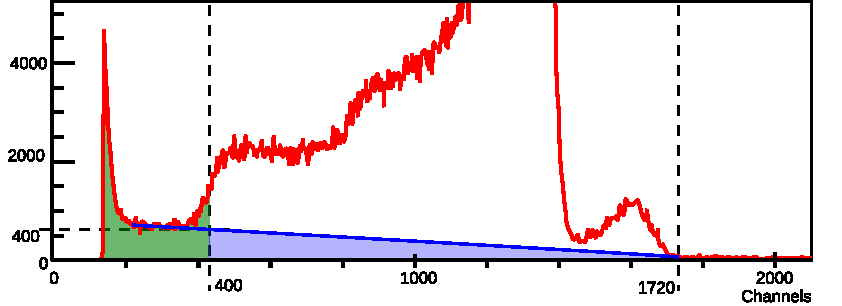
\includegraphics[width=0.8\textwidth]{BF3background.pdf}
  \caption{An estimate of the background is made by assuming it falls linearly from the beginning of the channel numbers, which has to be error, to a point where it is known to be zero, after the second peak. The green shaded region is known to background since the second step represents the loss of both the lithium and the $\alpha$ particles. \label{fig:bf3errorest}}
\end{figure}

The total number of counts is a function provided by the software that is used, called Maestro. This allows us to easily record the number of counts for specific regions of the graph. Using this method, and initial trial recording was taken to work out an estimate for the percentage of the total counts were contributed by this background radiation. Equation~\ref{eq:backgroundcalc} shows the calculation used to calculate the background,
\begin{align}
  (1729-400)\times 400 \times 0.5 &= 264,000\,\text{counts} \label{eq:backgroundcalc}
\end{align}
The total counts, including this noise, was $3.82\times10^6$, hence, the background represents roughly 6.9\% of the total counts.
% subsection neutron_attenuation (end)

\subsection{Neutron Attenuation Theory} % (fold)
\label{sub:neutron_attenuation_theory}
In order to model the situation, in a simplified way, the statistical one-group approach is used. It shall be assumed that all of the neutrons are thermalized, reduced in speed to similar to the surrounding particles, and an estimate for the diffusion length can be found. The diffusion length is the distance a thermal, or fast travelling neutron, takes to slow down. Once it has been thermalised, the neutron can be absorbed by matter, for example, an oxygen atom in the water surrounding the source. Thermalization is the best method for reducing the speed of neutrons for many applications, since neutrons are not charged particles and so do not interact with electric or magnetic fields.

The Americium-Beryllium source that was used was assumed to be a point source, which is a good approximation compared with the distances that we are measuring, and so the emitting of neutrons from such a source is given by
\begin{align}
  \dx{n}{t} &= -\Sigma_a \phi - \div{J} \label{eq:neutronflux}
\end{align}
where $n$ is the number of neutrons at time $t$, $\Sigma_a$ is the absorption cross section of the water in the tank, $\phi$ is the neutron flux (number of neutrons travelling through a unit are in unit time) and the vector $\textbf{J}$ is the diffusion flux from Fick's law shown in equation~\ref{eq:fick},
\begin{align}
  \textbf{J} = - \textbf{D}\grad\phi \label{eq:fick}
\end{align}
This means that the term from equation~\ref{eq:neutronflux}, $-\Sigma_a\phi$ is the loss of neutrons due to absorption, and the term $-\div{\textbf{J}}$ is the divergence. Since the flux is simply the number passing a static point multiplied by their velocity, $\phi = nv$, equation~\ref{eq:neutronflux} can be written as
\begin{align}
  \frac{1}{v}\dx{\phi}{t} &= -\Sigma_a\phi + D\laplacian\phi^2
  \intertext{But in the steady state, $\dx{\phi}{t} = 0$, so}
  \Sigma_a\phi &= D\laplacian\phi
\end{align}
The region of interest around the source, the water tank filled with water, has cylindrical symmetry but also, up to a radius of roughly 0.5\,m has spherical symmetry. In this case, the neutron flux is independent of the angle measured at and so this equation can be simplified to to a single dimension.
\begin{align}
  \frac{1}{r^2}\frac{\text{d}}{\text{d}r^2}\left( r^2\dx{\phi_r}{r} - \frac{1}{L^2}\phi_r \right) &= 0 \label{eq:diffusion}
\end{align}
  where the diffusion length, L, which is the distance travelled by an average neutron through the water, is given by
\begin{align}
  L &= \sqrt{\frac{D}{\Sigma_a}}.
\end{align}
The solutions of the equation~\ref{eq:diffusion} have the form
\begin{align}
  \phi &= A\frac{e^{-\frac{r}{L}}}{r} + B\frac{e^{\frac{r}{L}}}{r}
\end{align}
To simplify this equation, it is assumed that the coefficient, $B$, is zero, since otherwise the second term would tend to infinity as the radius increases, which is clearly un-physical. This leaves the following equation
\begin{align}
  \phi &= A\frac{e^{-\frac{r}{L}}}{r} \\
  r\phi &\propto e^{-\frac{r}{L}}
\end{align}
Thus, when $\ln(r\phi)$ is plotted against $r$, the graph should have a gradient of $-\frac{1}{L}$\cite{krane}. The equation here uses the flux of neutrons, $\phi$, which is the number of neutrons per unit area per unit time. However, since the measurements for the different positions of the detector were all taken using the same equipment, and for exactly the same time duration, this can be equally considered to be the total neutron count when considering the trend as the detector is moved.
% subsection neutron_attenuation_theory (end)
% section neutron_attenuation_in_water (end)

\subsection{Experimental Results} % (fold)
\label{sub:bf3experimental_results}
The data in table~\ref{tab:bf3results} is from the experiment to measure how the attenuation of neutrons is affected by a moderator, in this case water, as a function of distance. The data was taken using the Boron-triflouride detector suspended in the water at a position $r$ from the source. The detector was used to take a count of the number of neutrons from the source in a 10 minute interval, and then moved to the next position where the count was retaken.
\begin{table}[ht]
  \centering
  \begin{tabular}{c|c}
  Radius (m)  &   Counts   \\
  \hline\hline
  0.08        &   3.82E+06 \\
  0.10        &   3.10E+06 \\
  0.12        &   2.29E+06 \\
  0.14        &   1.64E+06 \\
  0.16        &   1.16E+06 \\
  0.18        &   8.18E+05 \\
  0.20        &   5.76E+05 \\
  0.22        &   3.98E+05 \\
  0.24        &   2.80E+05 \\
  0.26        &   1.97E+05 \\
  0.28        &   1.40E+05 \\  
  \end{tabular}
  \caption{The experimental data for the BF$_3$ was taken by moving the detector a given distance after measuring the neutron tank for 10 minutes.\label{tab:bf3results}}
\end{table}

These data are plotted in the graph in figure~\ref{fig:bf3data1} which shows the channel number plotted against the logarithm of the count number. This roughly fits the straight line fit showing that there is an exponential decrease in the number of neutrons reaching the detector as the detector is moved away from the source. The fit is not good, however, for the first two data points. These show a number of counts considerably below the expected result if it were to follow the straight line fit. If these two points are removed, and the data fit again to the straight line, the fit becomes much better. This effect can be seen in figure~\ref{fig:bf3data2}. 
\begin{figure}[ht]
  \centering
  \begin{subfigure}[b]{0.48\textwidth}
    \centering
    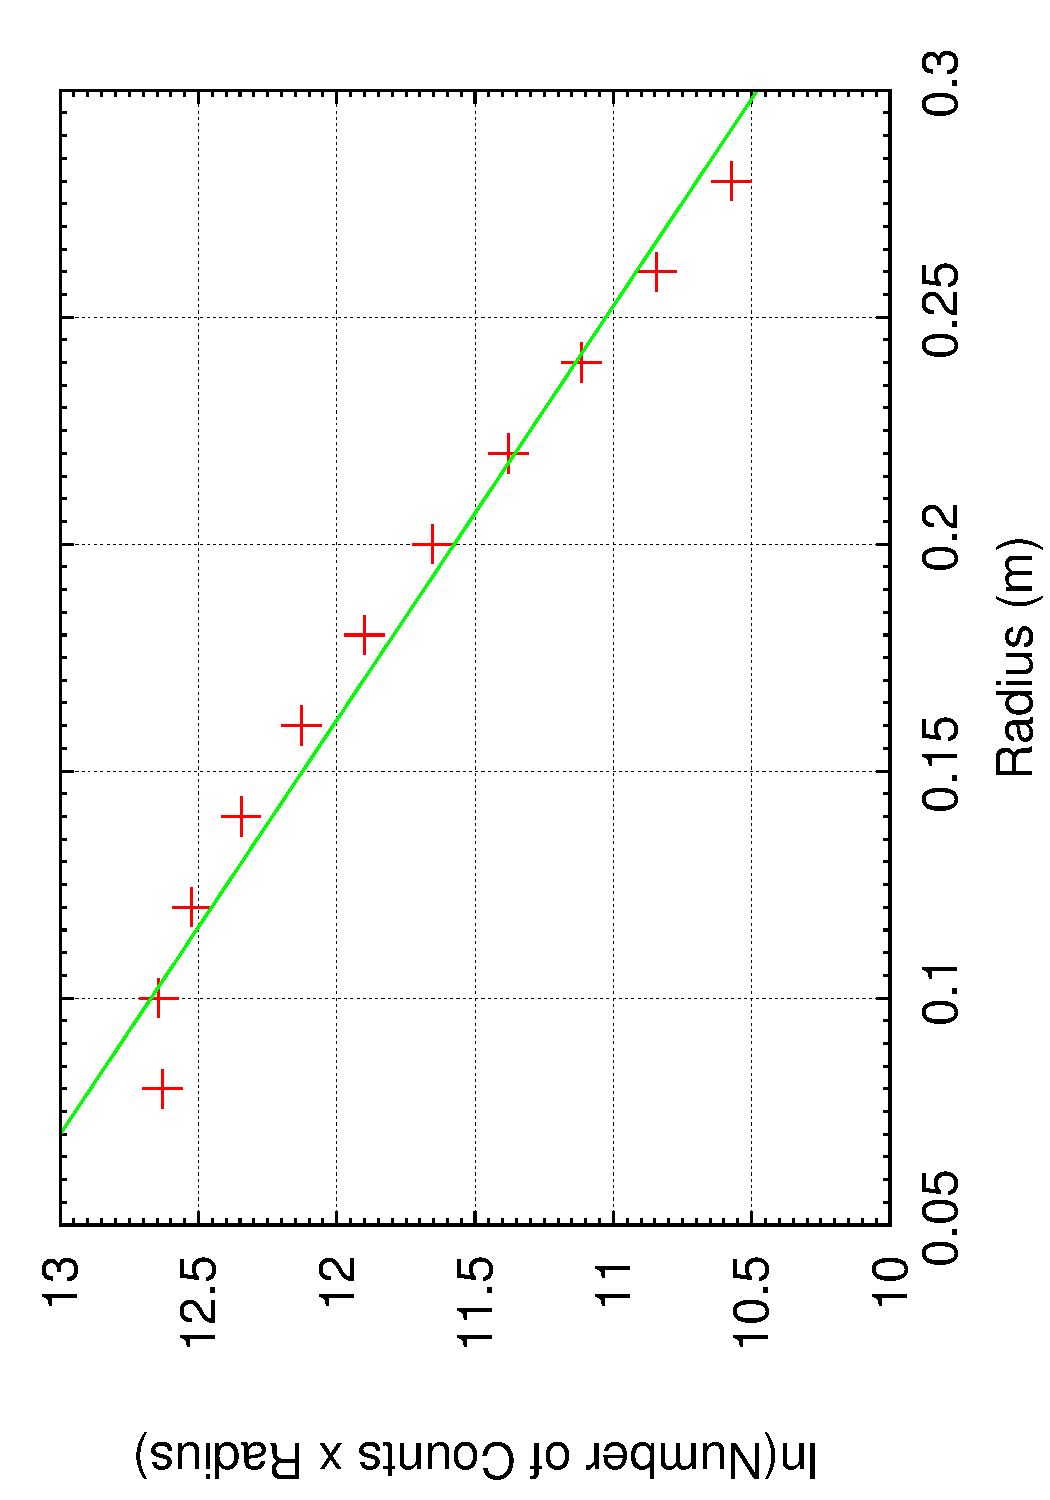
\includegraphics[angle=270,width=\textwidth]{BF3data1.pdf}
    \caption{The data from the BF$_3$ detector when plotted as the distance from the source against the logarithm of the number of counts gives a straight line, but two points do not seem to follow the general trend.\label{fig:bf3data1}}
  \end{subfigure}
  ~
  \begin{subfigure}[b]{0.48\textwidth}
   \centering
    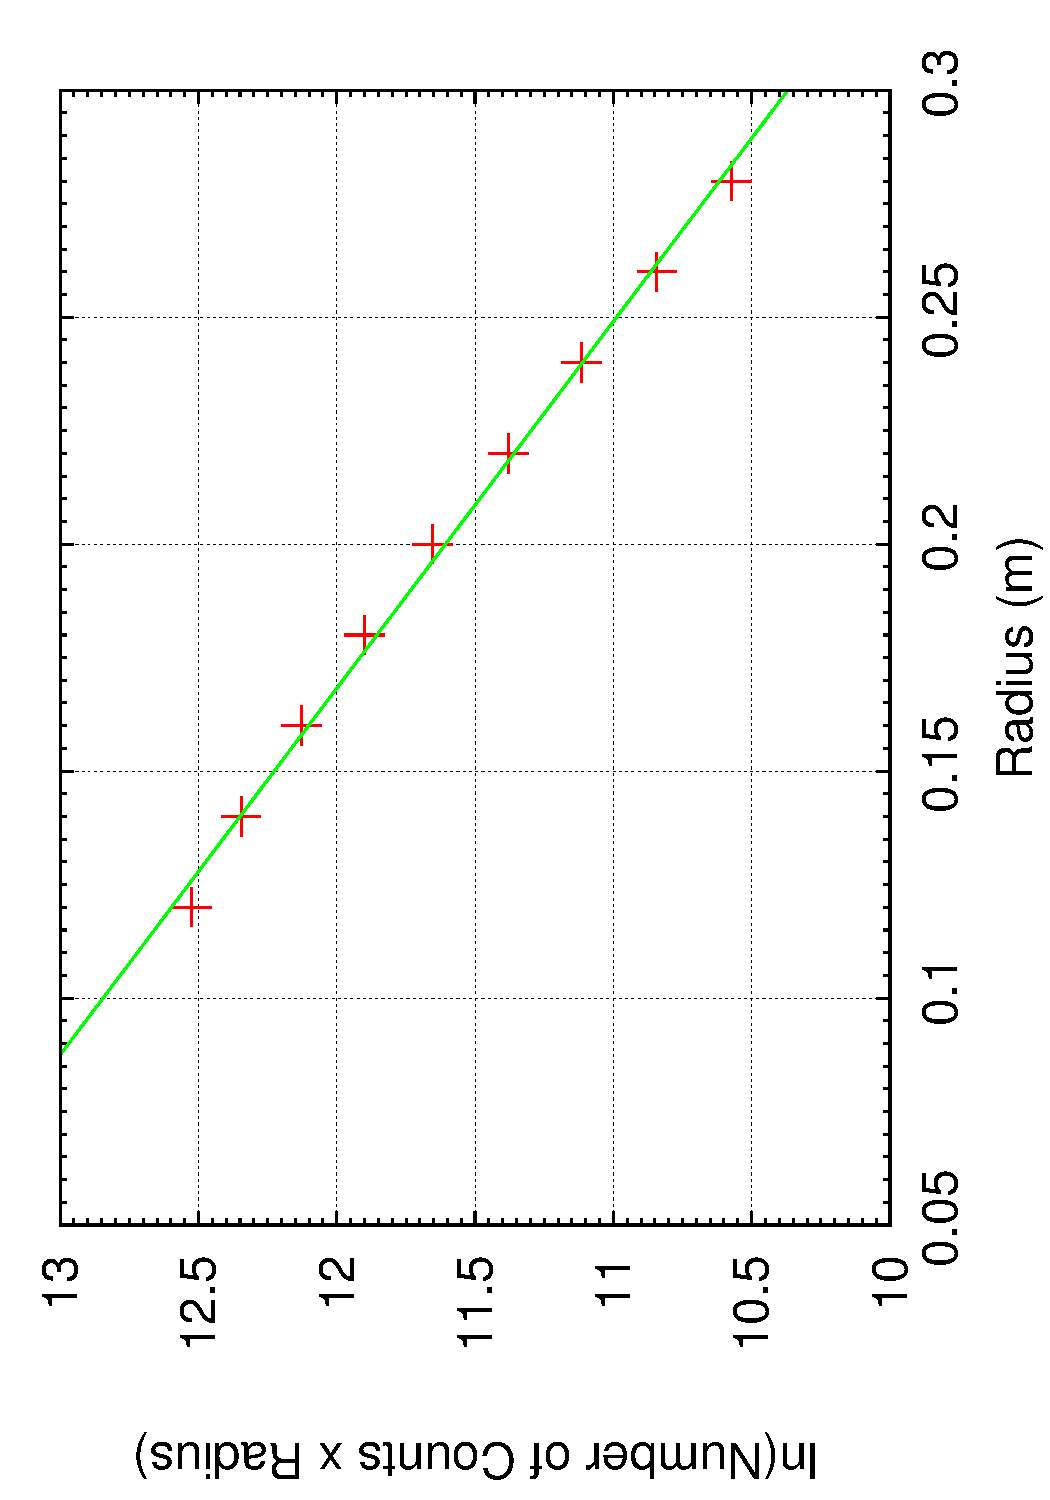
\includegraphics[angle=270,width=\textwidth]{BF3data2.pdf}
    \caption{If the two points are removed, the straight line fit is much more accurate. These data points are due to the distance over which a thermal neutron is slowed down sufficiently for the detector to observe it. \label{fig:bf3data2}}
  \end{subfigure}
  \caption{BF$_3$ data showing the linear relation when plotted as $\ln(\phi\times r)$ against $r$}
\end{figure}

This discrepancy from the expected trend close to the source can be explained by considering the distance from the source that the detector is for these two readings. These readings are for the distances 8\,cm and 10\,cm. At these distances, the thermal neutrons that are produced by the source have not had enough distance in the moderator to be thermalized. The BF$_3$ detector has a much smaller cross section for thermal neutrons than it does for slower neutrons, and so fewer of the neutrons that approach the detector at these distances are measured, even though there are more of them.

To explain, mathematically, this process would require the two-group version of the equation above. This has the form
\begin{align}
  \phi &= \frac{SL_T^2}{4\pi r \bar{D} (L_T^2 - \tau_T)} \left( e^{-r/L_T} - e^{-r/\sqrt{\tau_T}} \right) 
\end{align}
where 
\begin{itemize} \itemsep1pt \parskip0pt \parsep0pt
  \item $S$ is the source strength
  \item $L_T^2$ is the neutron diffusion length
  \item $\bar{D}$ is the diffusion constant
  \item $\tau_T$ is the neutron age
\end{itemize}
An attempt was made to solve this problem using the 

We can also plot the data points as counts against the radial distance from the source, as shown in figure~\ref{fig:bf3countsvsradius}. As can be seen, this provides a rough exponential decrease in the recorded counts as the distance from the source increases. The relevant data is also shown below, table~\ref{tab:bf3data}. This table also shows the values that were used to calculate the background that was present in each measurement, as described in section~\ref{sub:neutron_attenuation}.
\begin{align}
  \text{total background} = (\text{max. channel} - \text{min. channel}) \times \text{est. background} \times \frac{1}{2}
\end{align}
\begin{figure}[ht]
  \centering
  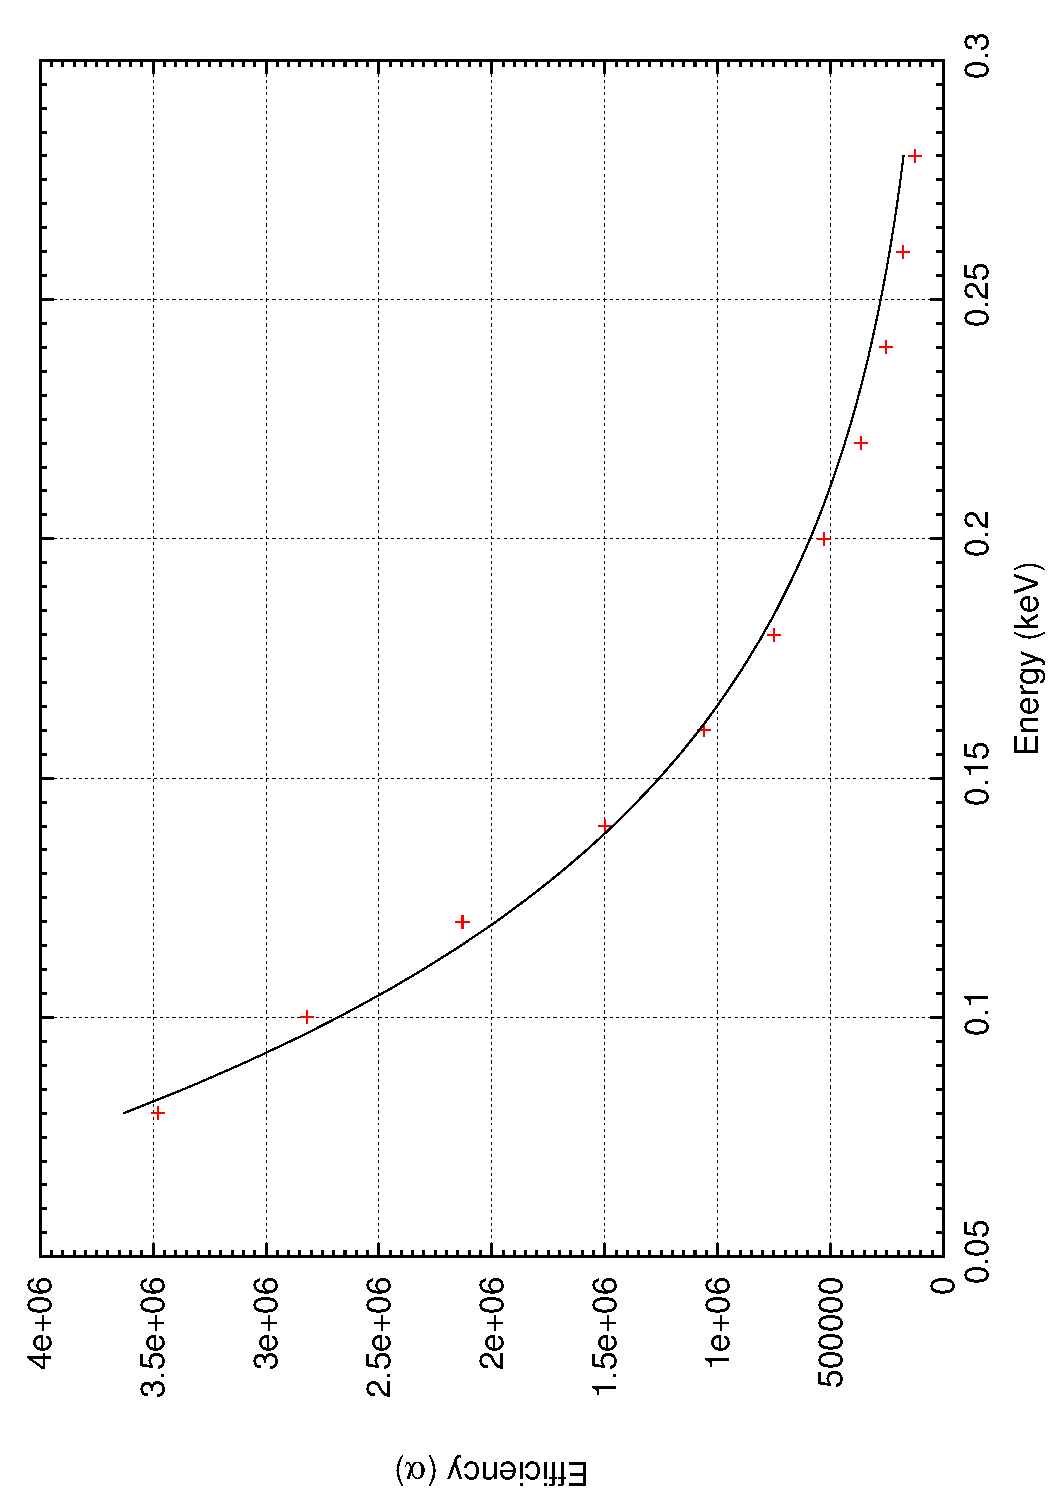
\includegraphics[angle=270,width=0.8\textwidth]{BF3countsvsradius.pdf}
  \caption{An estimate of the background is made by assuming it falls linearly from the beginning of the channel numbers, which has to be error, to a point where it is known to be zero, after the second peak. The green shaded region is known to background since the second step represents the loss of both the lithium and the $\alpha$ particles. \label{fig:bf3countsvsradius}}
\end{figure}
\begin{table}[ht]
  \centering
  % \begin{tabular}{c|m{2em}|m{4em}|m{2em}|m{4em}|m{5em}|c|c}
  \begin{tabular}{L|M|O|M|O|N|N|c}
    Radius (m)  &Min Chn  &Est Backgnd  &Max Chn  &Est Backgnd  &Overall Backgnd  &Counts   &Counts-Backgnd \\
    \hline\hline
    0.08  &407    &480    &1734   &37       &$3.43\times 10^{05}$     &$3.82\times 10^{06}$ &$3.48\times 10^{06}$     \\
    0.10  &400    &390    &1752   &17       &$2.75\times 10^{05}$     &$3.10\times 10^{06}$ &$2.82\times 10^{06}$     \\
    0.12  &399    &220    &1755   &19       &$1.62\times 10^{05}$     &$2.29\times 10^{06}$ &$2.13\times 10^{06}$     \\
    0.14  &405    &200    &1768   &6.4      &$1.41\times 10^{05}$     &$1.64\times 10^{06}$ &$1.50\times 10^{06}$     \\
    0.16  &401    &140    &1757   &3.6      &$9.74\times 10^{04}$     &$1.16\times 10^{06}$ &$1.06\times 10^{06}$     \\
    0.18  &409    &100    &1759   &1.6      &$6.86\times 10^{04}$     &$8.18\times 10^{05}$ &$7.49\times 10^{05}$     \\
    0.20  &398    &70.0   &1757   &0.83     &$4.81\times 10^{04}$     &$5.76\times 10^{05}$ &$5.28\times 10^{05}$     \\
    0.22  &402    &50.0   &1756   &0.43     &$3.41\times 10^{04}$     &$3.98\times 10^{05}$ &$3.64\times 10^{05}$     \\
    0.24  &405    &35.0   &1759   &0.18     &$2.38\times 10^{04}$     &$2.80\times 10^{05}$ &$2.56\times 10^{05}$     \\
    0.26  &403    &25.0   &1752   &0.16     &$1.70\times 10^{04}$     &$1.97\times 10^{05}$ &$1.80\times 10^{05}$     \\
    0.28  &408    &18.0   &1749   &0.12     &$1.21\times 10^{04}$     &$1.40\times 10^{05}$ &$1.27\times 10^{05}$     \\
  \end{tabular}
  \caption{This table shows the values for the BF$_3$ experiment. The count number is shown as a function of the radial distance from the source, as well as the estimated background for each of these readings calculated from the known background at the start and end of the spectrum and then using equation~\ref{eq:backgroundcalc}.\label{tab:bf3data}}
\end{table}

% subsection experimental_results (end)
